This section describes the analysis methodology. We use boosted $Z\to\tauhad\taulep$ events to measure Monte Carlo correction factors for the tau identification algorithms in the high-$\pt$ region.

Different working points are defined for RNN score relative to the efficiency of selecting true $\tauhad$ candidates. When the efficiency of the working points is measured in data and simulation, a correction factor has to be derived and then applied to the simulation in order for the signal efficiency to agree between data and simulation \cite{ATLAS:2017mpa}. Because of the top quark mass, $t\bar{t}$ events are usually used as a source of high momentum taus for measuring correction factors on the high-$p_T$ bins. However, Lepton universality may not hold in W decays. For that reason our study is aimed to use boosted $Z\to\tauhad\taulep$ events for deriving and cross checking the simulation correction factors in the high-$p_T$ region.   
\subsection{Signal events}\label{signalevents}
For this study, we consider as signal events where one the taus decays hadronically and the other leptonically, either into an electron or a muon. Thus, our final states will include a $\tauhad$ candidate and a lepton $l=e,\mu$. The presence of the light lepton will be used as our tag. 
Generally, in $\Zll$ events, the taus are produced back to back and their $\pt$ spectrum falls sharply. One way to select events where the taus are boosted in the transverse plane is to look for events where the opening angle in the transverse plane between the taus ($\Delta\phi(\tauhad,\taulep)$) is more acute. A depiction of the topologies of our signal events is shown in Fig.\ref{Fig1}. For these events, the missing transverse momentum ($\met$) is assumed to come from the neutrinos produced in the decays of the tau leptons. Due to the fact that two neutrinos are produced in the leptonic decay mode we expect our events to have a larger $\met$ component along the $\taulep$ direction.
\begin{figure}[htbp]
	\centering
	\subfloat[]{\label{Fig1a}{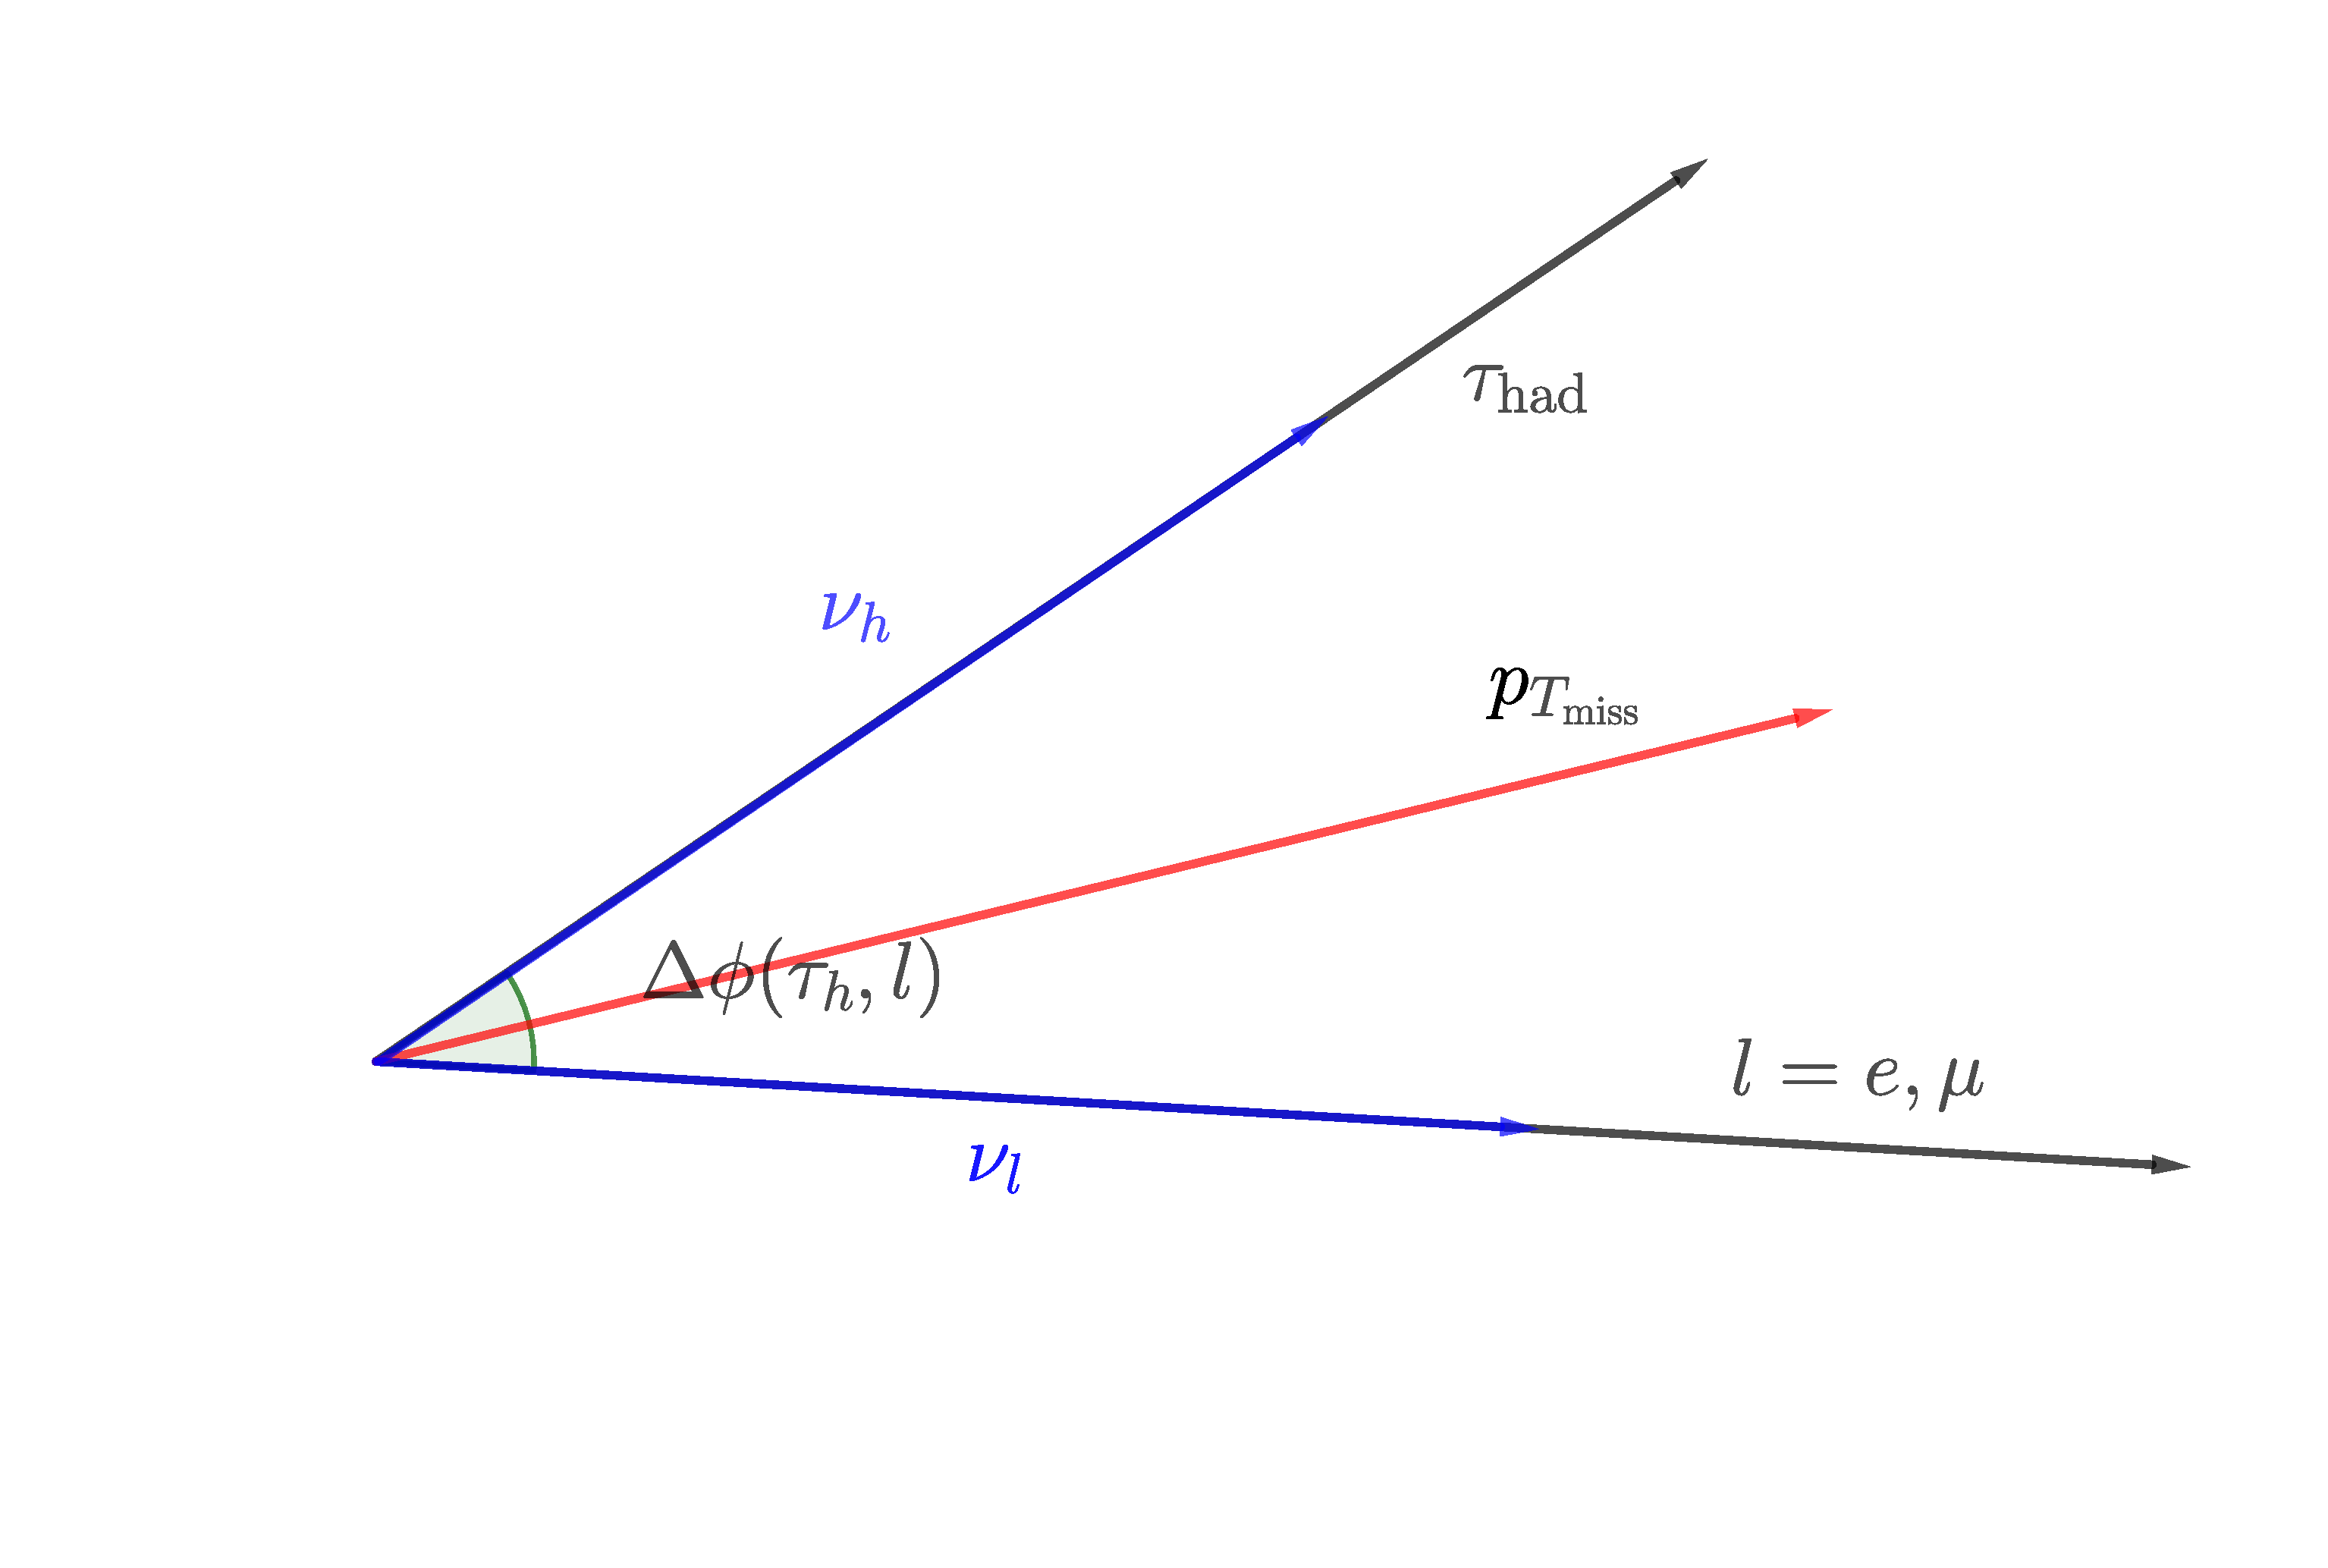
\includegraphics[width=0.49\textwidth]{Fig1a}}}\hfill
	\subfloat[]{\label{Fig1b}{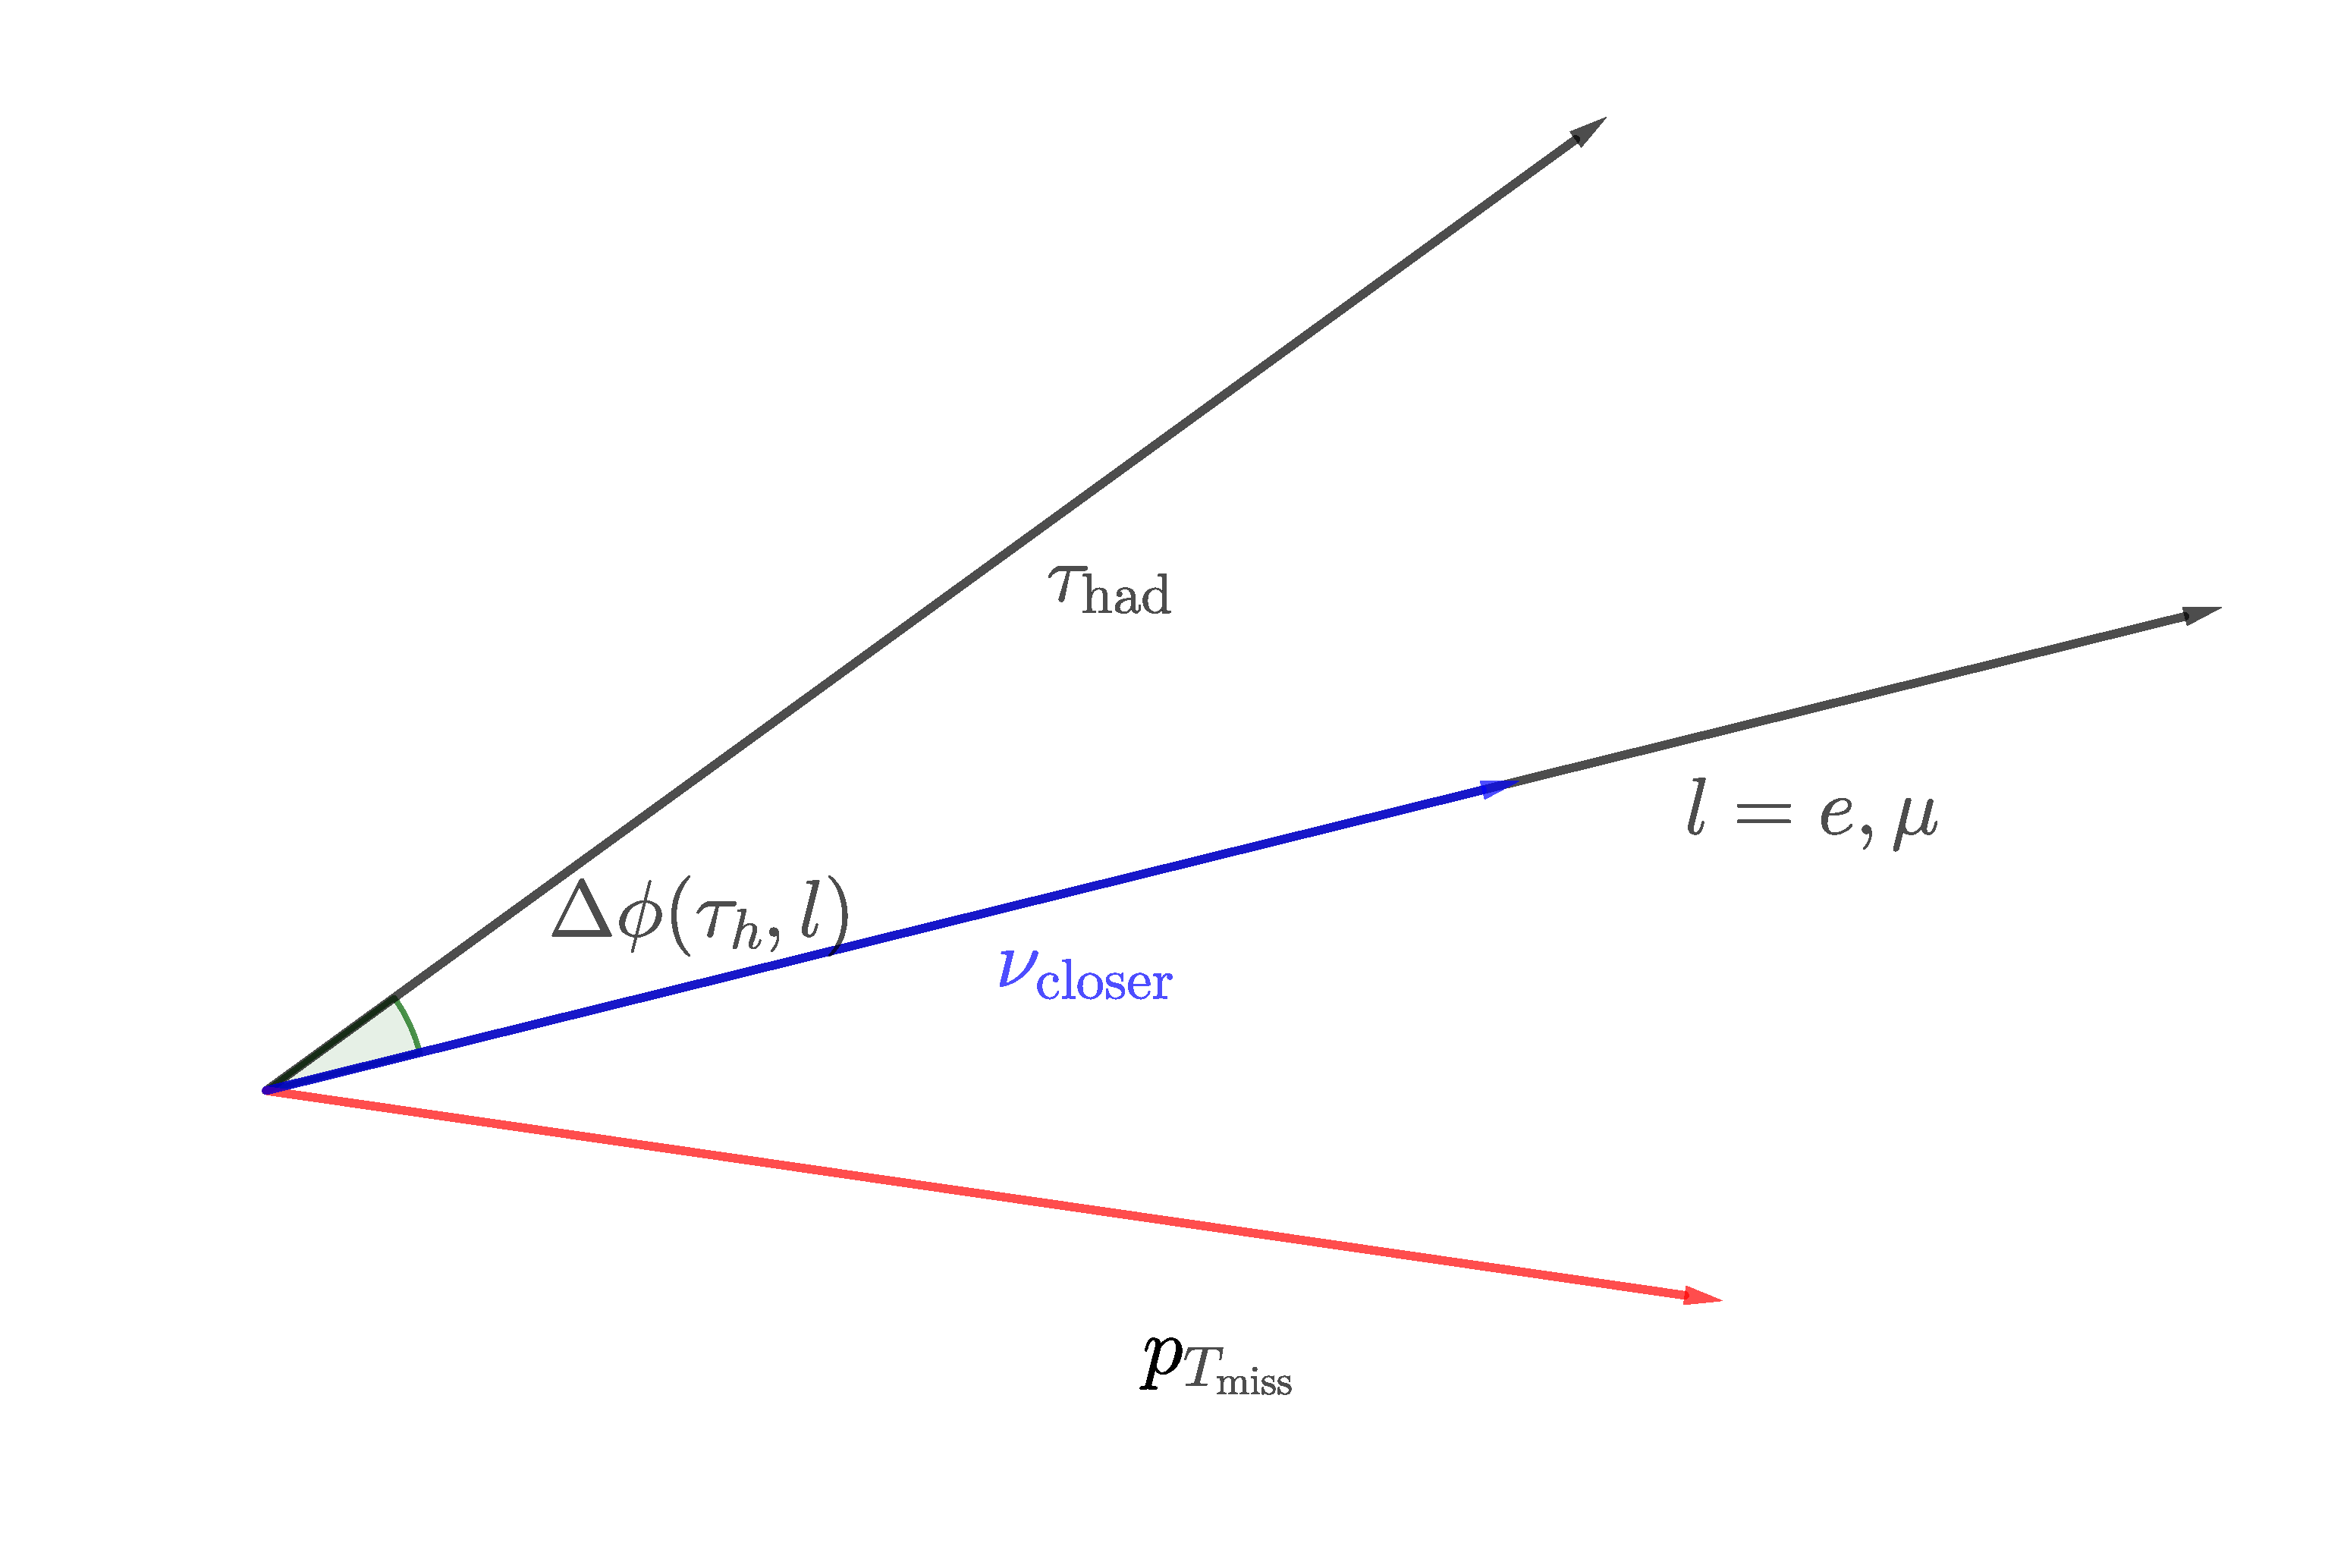
\includegraphics[width=0.49\textwidth]{Fig1b}}}
	\caption{The two different types of topologies that define signal events. On the left, when the missing energy is between the visible objects two neutrinos are assumed to be responsible for all the missing energy. On the right, only one neutrino is assumed to be flying on the direction of the visible object closest to the missing energy.}
	\label{Fig1}
\end{figure}